\section{Introduction}
The Standard Model includes three charged leptons, three neutrinos and six quarks and their antiparticles which are splitted into three generations and can interact through gauge bosons (see \ref{fig:StandardModel}). The neutrinos. neutrinos are fundamental particles of the Standard Model.\ref{ref_PDG}\\
Figure with Standard Model particles and interations. \\

\begin{figure}
\caption{Fundamental particles and interactions}
\label{fig:StandardModel}
\centering
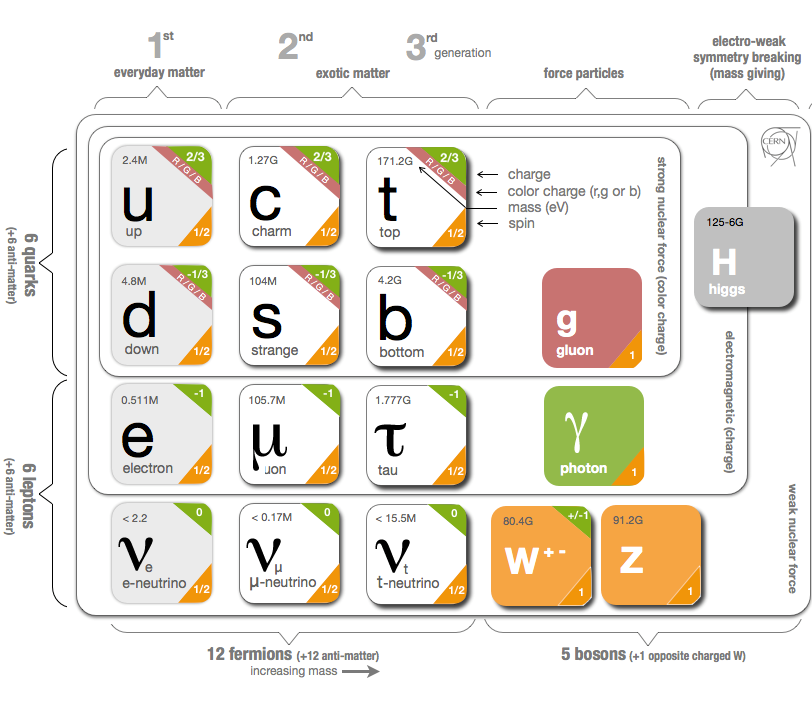
\includegraphics[width=0.8\textwidth, keepaspectratio=true]{figs/StandardModel.png}
\\Three generations of fundamental particles and interaction mediators. Charged leptons and quarks are subjects to electromagnetic interactions (through photons). Quarks can also interact strongly (through gluons). All leptons and quarks can interact weakly (through $W^{\pm}$ and $Z^0$ bosons). All the particles shown are discovered at the moment and no other fundamental particle is discovered. \cite{ref_fig_StandardModel}   
\end{figure}

How many neutrinos pass through the $cm^2$ per second (flux), check PDG.\\
Two very common and well known interactions which includes neutrinos are neutron beta decay and muon decay. The Feynmann diagrams of these processes are shown at \ref{fig:MuonAndNeutronBetaDecays}. Mean lifetime of free neutron is $~15$ minutes and $>99.9\%$ of those which decay will do it though the beta decay: $n \rightarrow p + e^- + \bar{{\nu}_e} $ \cite{ref_PDG}. At the level of fundamental particles, neutron consists of two d-quarks and one u-quark and in the beta decay one of the d-quarks transfers to u-quark though the weak interaction mediated by $W^- $ boson. Thus, the proton, which consists of two u-quark and one d-quark, is being produced. When this happens, the electron and electron antineutrino are emitted to preserve the charge and the lepton Flavor number conserved. The examples of the neutron beta decay in nature include ${^{49}}{_{19}}K \rightarrow {^{40}}{_{20}}Ca$, ${^{64}}{_{29}}Cu \rightarrow {^{64}}{_{30}}Zn$, ${^3}{_1}H \rightarrow {^3}{_2}He$ \cite{ref_Griffiths} (the positive beta decay,  $p \rightarrow n + e^+ + {\nu}_e $, is not possible for free proton but it can happen when the proton is the part of the nuclei). As for the muon, it's mean lifetime is $~2 {\mu}s$ and $~99\%$ of muons which decay would do that to electron, nuom neutrino and electron antineutrino as ${\mu}^- \rightarrow e^- + {\nu}_{\mu} + \bar{{\nu}_e}$ though the the W boson. This process is also common in nature, in cosmic rays: muon are produced in the upper layers of the Earth atmosphere from the interaction of the particles coming from cosmics with the atmosphere substances though the reaction [WHICH REACTION ?] and then some number of muons decay while traveling through the atmosphere to the ground.   

\begin{figure}
\caption{Feynmann diagrams of neutron and muon decays}
\label{fig:MuonAndNeutronDecays}
\centering
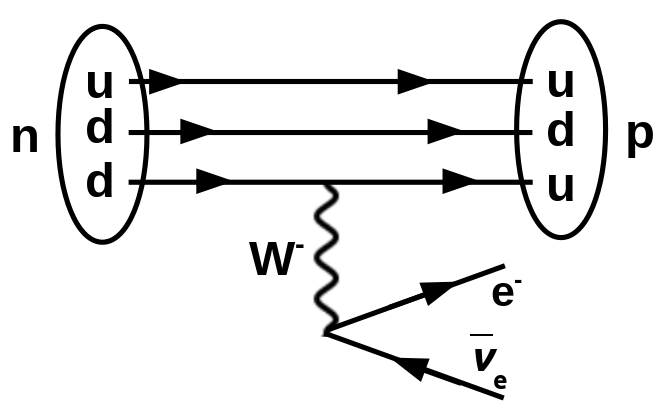
\includegraphics[width=0.3\textwidth, keepaspectratio=true]{figs/NeutronBetaDecay.png}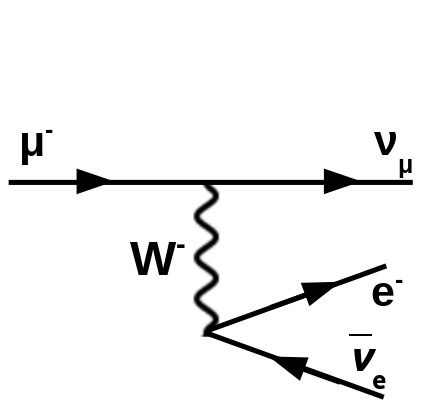
\includegraphics[width=0.3\textwidth, keepaspectratio=true]{figs/MuonDecay.png}
\\Feynmann diagrams of left: neutron beta decay \cite{ref_fig_NeutronDecay}(d-quark of transfers to u-quark through the W-boson with emission of electron and antineutrino), right:  muon decay \cite{ref_fig_MuonDecay}(muon decays to electron, neutrino and antineutrino through W-boson).
\end{figure}

There are three flavors of neutrino, one for each generation: electron neutrino, muon neutrino, tau neutrino. And in the processes described above (neutron beta decay and muon decay) the lepton flavor numbers $L_e, L_{\mu} and L_{\tau}$ are conserved. The table \ref{tab:LeptonFlavorNumber} shows the value of this number for all leptons and antileptons. 

\begin{table}[h]
  \begin{center}
  \caption{ Lepton Flavor Number}
  \begin{tabular}{|c|c|c|c|}
     particles & $L_e$ & $L_{\mu}$ & $L_{\tau}$ \\ \hline
     $e^-,\nu_e$ &  +1  &  0  &  0  \\ \hline 
     $e^+, \bar{\nu_e}$ &  -1  &  0  &  0  \\ \hline 
     $\mu^-,\nu_{\mu}$ &  0  &  +1  &  0  \\ \hline 
     $\mu^+, \bar{\nu_{\mu}}$ &  0  &  -1  &  0  \\ \hline 
     $\tau^-,\nu_{\tau}$ &  0  &  0  &  +1  \\ \hline 
     $\tau^+, \bar{\nu_{\tau}}$ &  0  &  0  &  -1  \\ \hline 
  \end{tabular}
  \label{tab:LeptonFlavorNumber}
  \end{center}
\end{table}
